\documentclass[a4paper]{article}

\usepackage[english]{babel}
\usepackage[utf8x]{inputenc}
\usepackage{amsmath}
\usepackage{graphicx}
\usepackage[colorinlistoftodos]{todonotes}
%\usepackage[margin=1in]{geometry}
\setlength{\parindent}{0pt}
\usepackage{url}
\usepackage{float}
\usepackage[section]{placeins}

\title{Numerical Methods With Matlab}

\author{Benjamin Goss}

\date{\today}

\begin{document}
\maketitle


\section{Numerical Solution of ODEs}
\subsection{Forward Euler Method}
\subsubsection{}
%Explanation of Forward Euler Method

Forward Euler Method is a method for solving ordinary differential equations, when they have set initial conditions. It works by moving the solution from $x_n$ to $x_{n+1} = x_n + h$, and then through the entire timespan up to the top limit in steps of $h$. 

%Show given ODE - Math mode

The ODE supplied to be solved is:
$$\frac{\mathrm{d}x}{\mathrm{d}t} = -2tx^2,$$ $$x(0) = 1$$
for $t \in [0,2]$, with step sizes 0.2, 0.1 and 0.05. 
The exact solution for this ODE is:

$$x(t) = \frac{1}{(1+t^2)},$$

which was given to allow the calculation of the error to be exact rather than approximated.

%Explain the different step sizes

The step size is the difference added to each approximation to move to the next approximation. Generally, the smaller the step size the better.

%IMAGE - Code euler method

\begin{figure}[H]
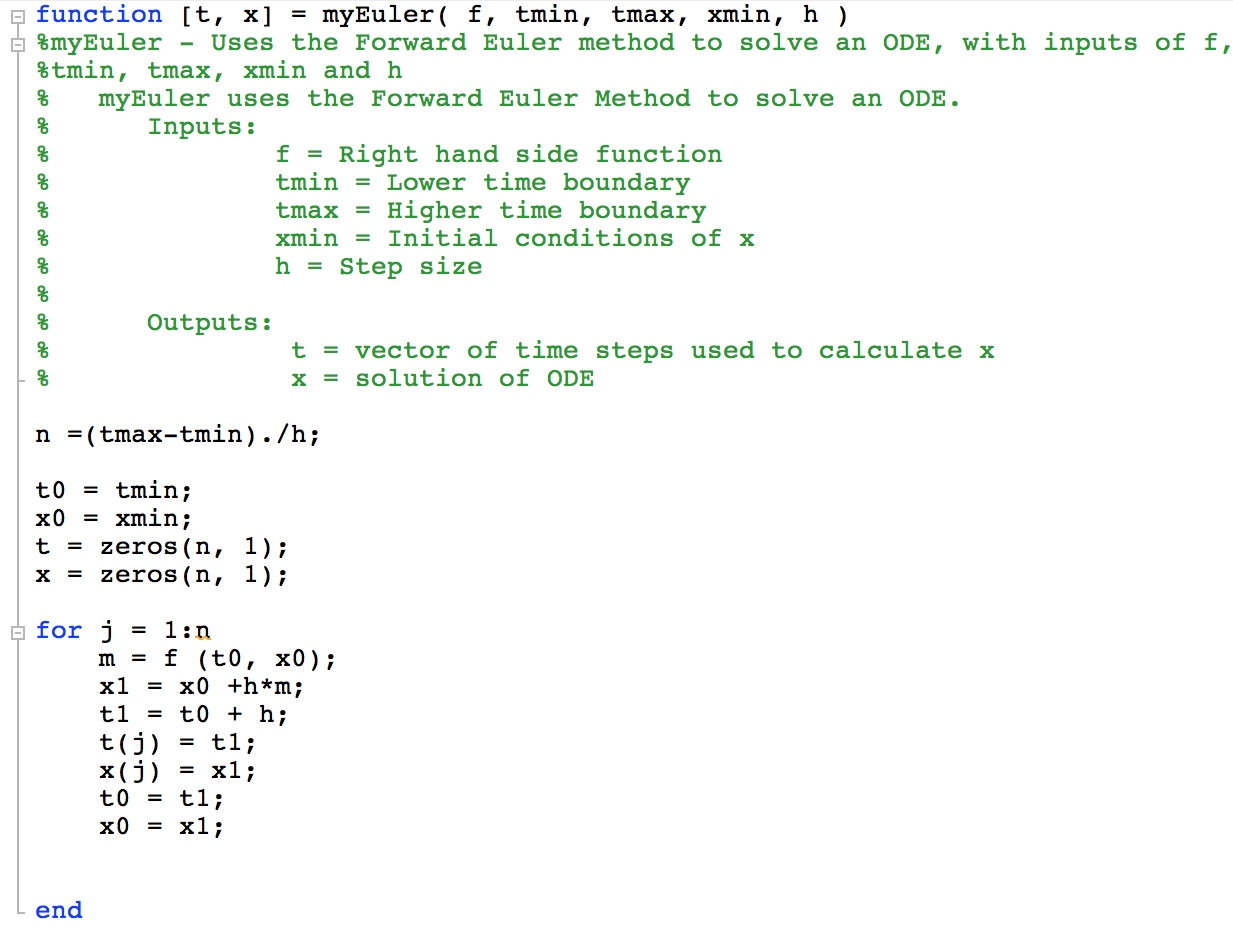
\includegraphics[width=1\textwidth]{myeuler.jpg}
\end{figure}
%Explanation of how the code works
The code shown above is a function for the forward Euler Method. It works by taking inputs of the right hand side function, the timespan, the initial values for x and the stepsize. It calculates the number of steps that need to be taken, and uses the right hand side function to create a vector of x values through the timespan, and a vector of t values in steps of h. 

\begin{figure}[H]
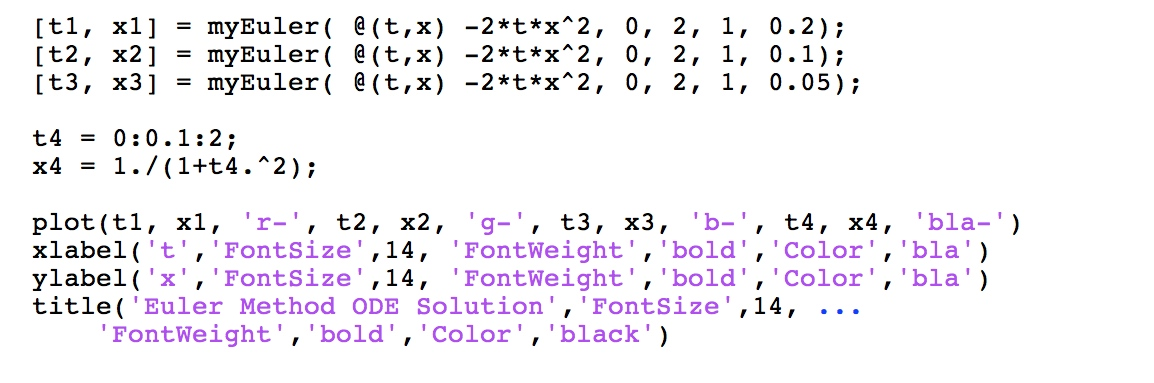
\includegraphics[width=1\textwidth]{question1ai.jpg}
\end{figure}
%Explanation of how the code works

This code is used to call the function myEuler for the ODE supplied, and plots the results on a graph. It also calculates the exact solution of the ODE. 
%IMAGE - Solutions graph

\begin{figure}[H]
\centering
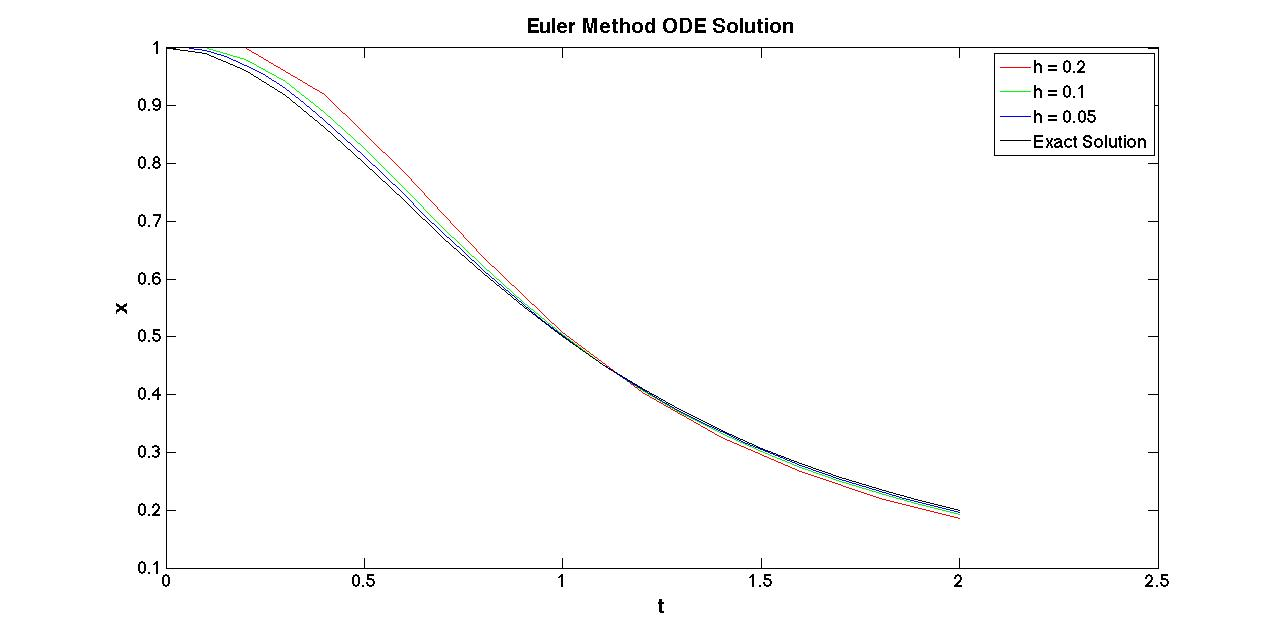
\includegraphics[width=1\textwidth]{eulerodesolution.jpg}
\caption{\label{fig:eulerodesolution}A graph showing the solutions to the ODE given above, with $t \in [0,2]$. }

\end{figure}

%Explain the solutions

As can be seen from Figure \ref{fig:eulerodesolution}, the numerical approximations to the solution follow the exact solution well, but the best approximation is $h = 0.05$, as it has the largest number of points, and thus has the smoothest curve. 

\subsubsection{}

%Explain absolute error

Absolute error is the difference between the approximated value, and the true value. As the true value for this ODE is given, the actual value of the absolute error can be used. 

%show the error values for the given step sizes
\begin{figure}[H]
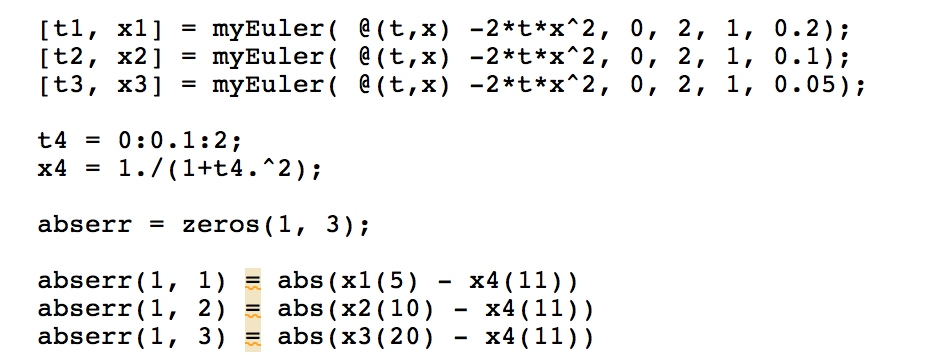
\includegraphics[width=1\textwidth]{question1error.jpg}
\end{figure}

Using the code shown above, it is possible to calculate the absolute error. The values that were returned by this code were 0.007060159605430, 0.003641976039014 and 0.001805472690540 for step sizes of 0.2, 0.1 and 0.05 respectively. 

%Explain how error would scale with h

As the values for the step size $h$ increase, generally the error decreases, as the smaller step size means less of a gap between the approximations values, and a much smoother curve. As the step size tends to zero, the error should also tend to zero, with the approximation converging with the exact solution.

%IMAGE - code for different step sizes

\begin{figure}[H]
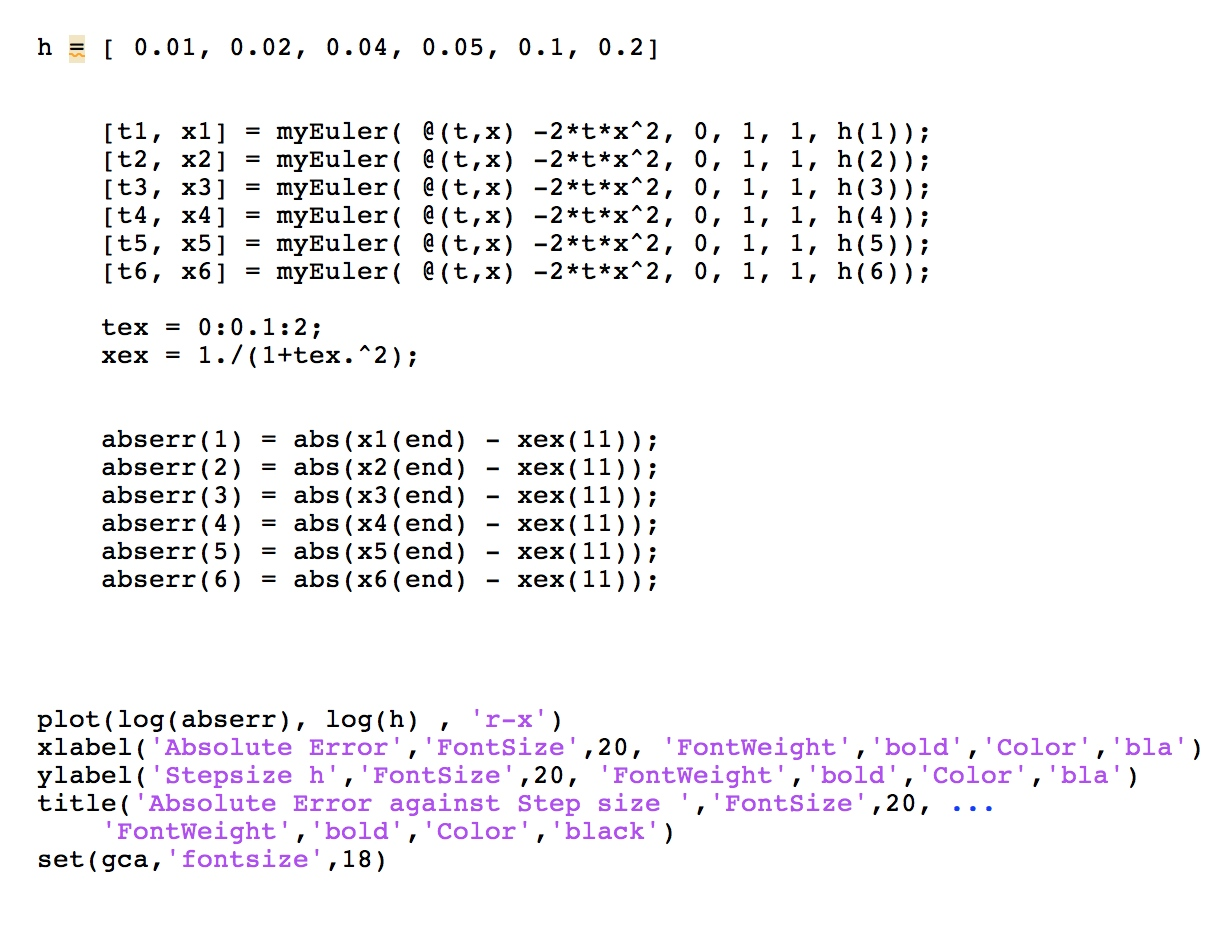
\includegraphics[width=1\textwidth]{ploterrorcode.jpg}
\end{figure}

The above code is used to calculate the absolute error for a variety of step sizes at time $t = 1$. 

%IMAGE - plot of error vs setp sizes from above

\begin{figure}[H]
\centering
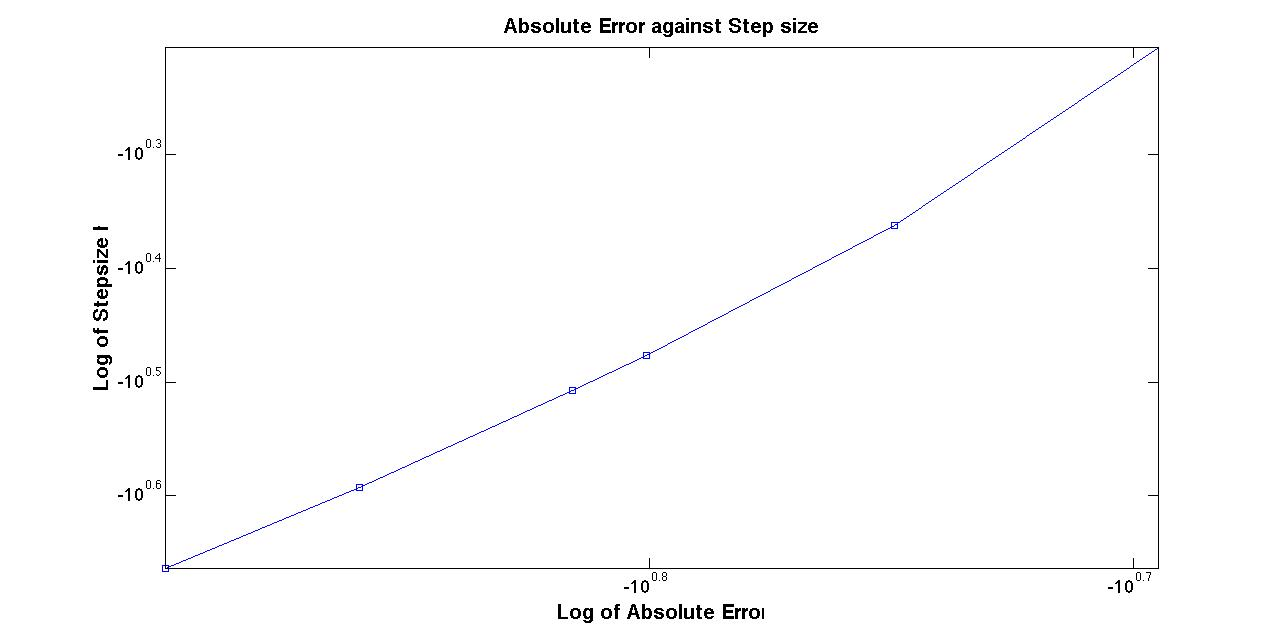
\includegraphics[width=1\textwidth]{question1errorstepsize.jpg}
\caption{\label{fig:question1errorstepsize}A loglog graph showing absolute error vs step size. }
\end{figure}
%Explain results

As can be seen from the Figure \ref{fig:question1errorstepsize}, as the log of the step size increases, as does the log of the absolute error. This means that as the step size decreases, the absolute error decreases, meaning that the approximation becomes more accurate as the step size increases. 

\subsection{Fourth Order Runge-Kutta}

%What is fourth order runge-kutta?

Fourth Order Runge-Kutta is another method for solving ODEs. It uses estimates of the slope in order to calculate the next step in the ODE. 

$$k_1 = f(t_n, y_n),$$
$$k_2 = f(t_n + \tfrac{h}{2}, y_n + \tfrac{h}{2} k_1),$$
$$k_3 = f(t_n + \tfrac{h}{2}, y_n + \tfrac{h}{2} k_2),$$
$$k_4 = f(t_n + h, y_n + hk_3).$$

The equations to estimate the slope are shown above. 

$$y_{n+1} = y_n + \tfrac{h}{6}\left(k_1 + 2k_2 + 2k_3 + k_4 \right)$$
$$t_{n+1} = t_n + h $$

The estimates of the slope are then used in the equation shown above, as a weighted average. This equation then gives the value of the next step of the ODE.
%IMAGE - code, myrungekutta

\begin{figure}[H]
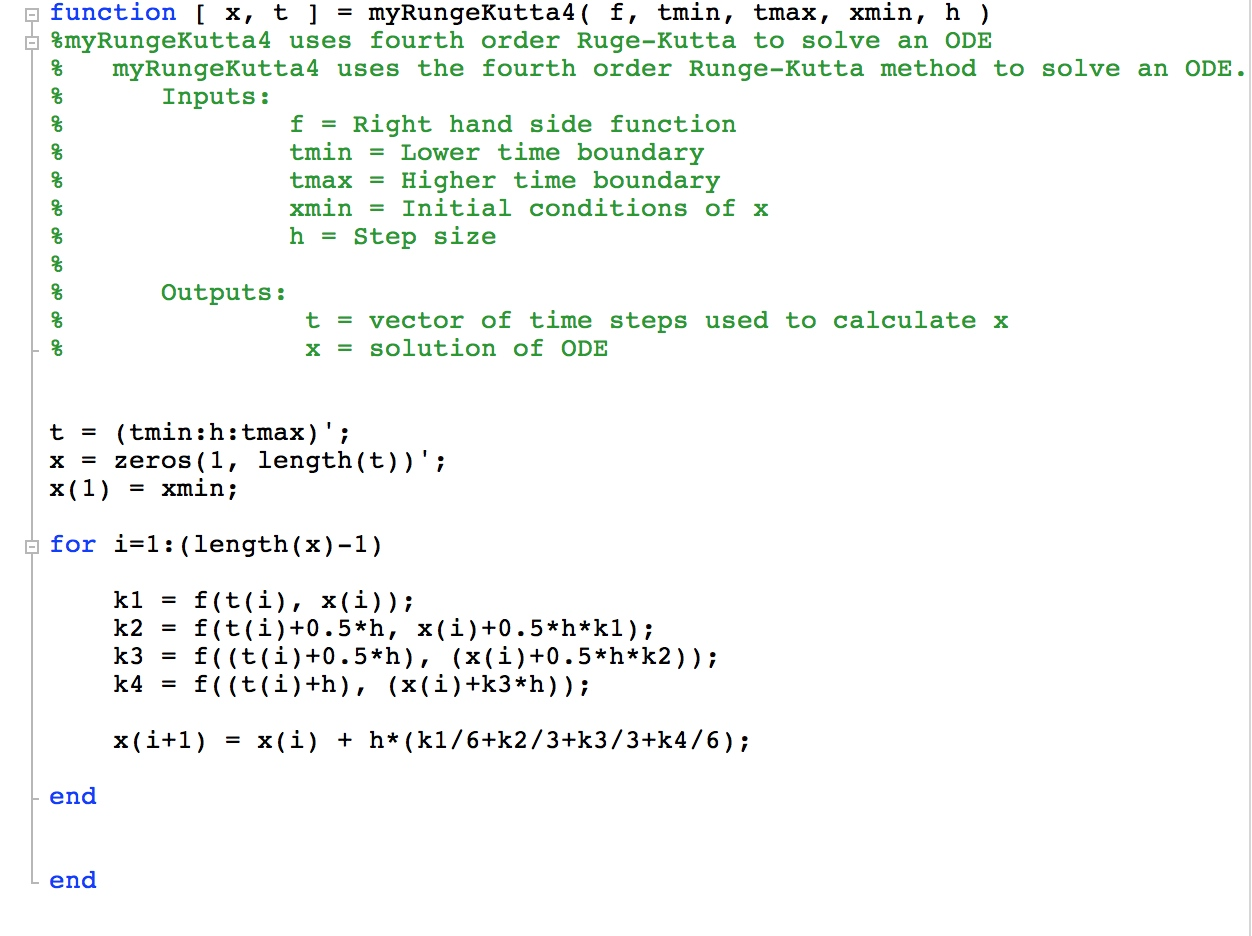
\includegraphics[width=1\textwidth]{myrungekuttacode.jpg}
\end{figure}

%Explain how the code works

The above code is the fourth order Runge-Kutta method implemented in Matlab. It takes five inputs; the right hand side function, the timespan, initial condition for x and the step size h. It then uses the Runge-Kutta equations to calculate the solution to the ODE. 

%IMAGE - code- question 1 calling myrungekutta

\begin{figure}[H]
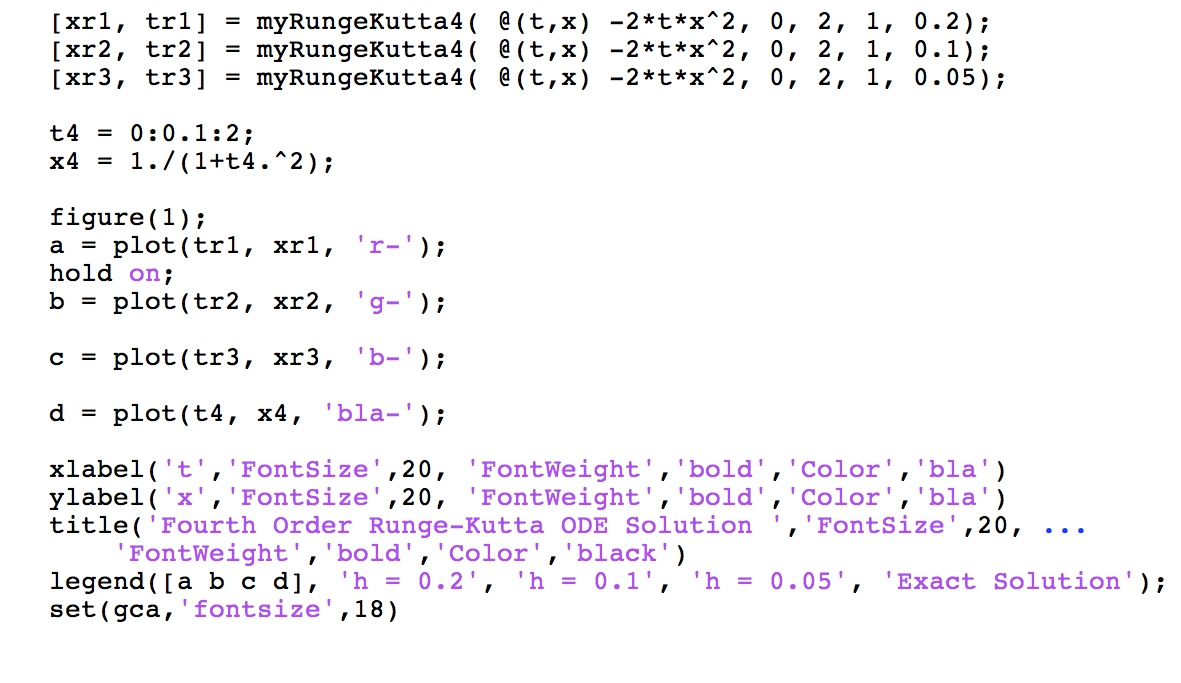
\includegraphics[width=1\textwidth]{rungekuttacode.jpg}
\end{figure}

%Explain code

This code calls the myRungeKutta4 function to solve the ODE that was given in part 1.1. It then plots the solutions for three different step sizes, as well as the exact solution. 

%IMAGE - solutions graph

\begin{figure}[H]
\centering
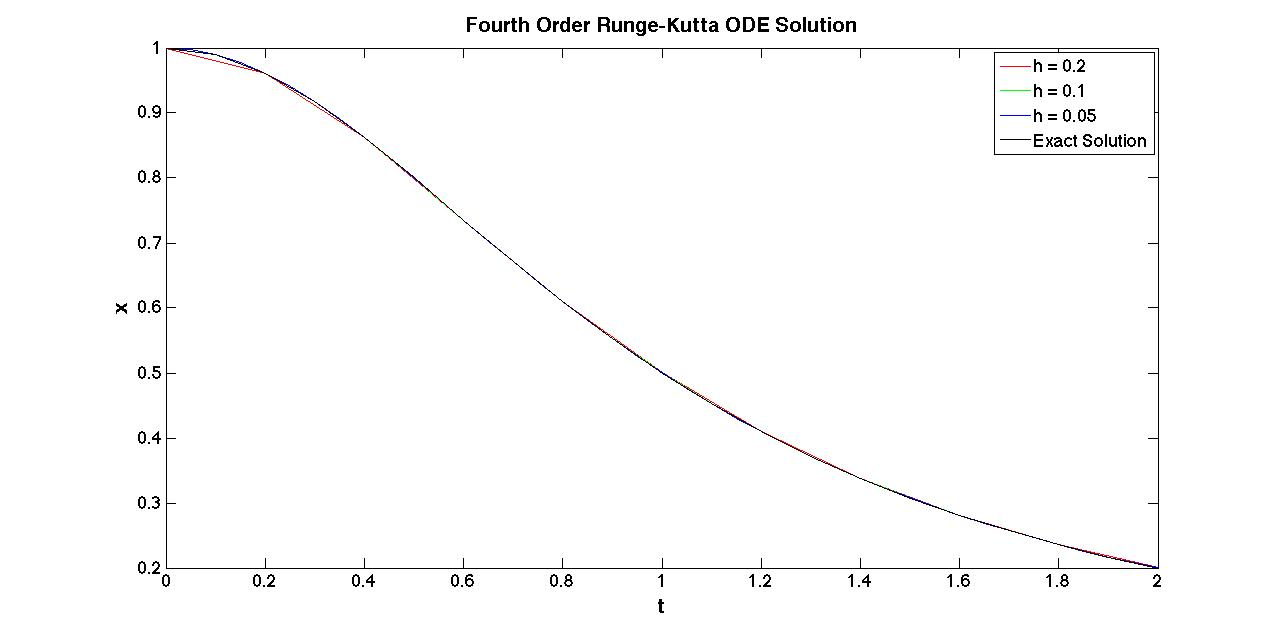
\includegraphics[width=1\textwidth]{rungekuttasolution.jpg}
\caption{\label{fig:rungekuttasolution}A graph showing the solutions to the ODE given above, with $t \in [0,2]$. }
\end{figure}

%Explain solutions

As can be seen in Figure \ref{fig:rungekuttasolution}, the solutions that are found from the fourth order Runge-Kutta method are incredibly close to the exact solution, much more so than the forward Euler method.  

%Explain how error should change with step size

\begin{figure}[H]
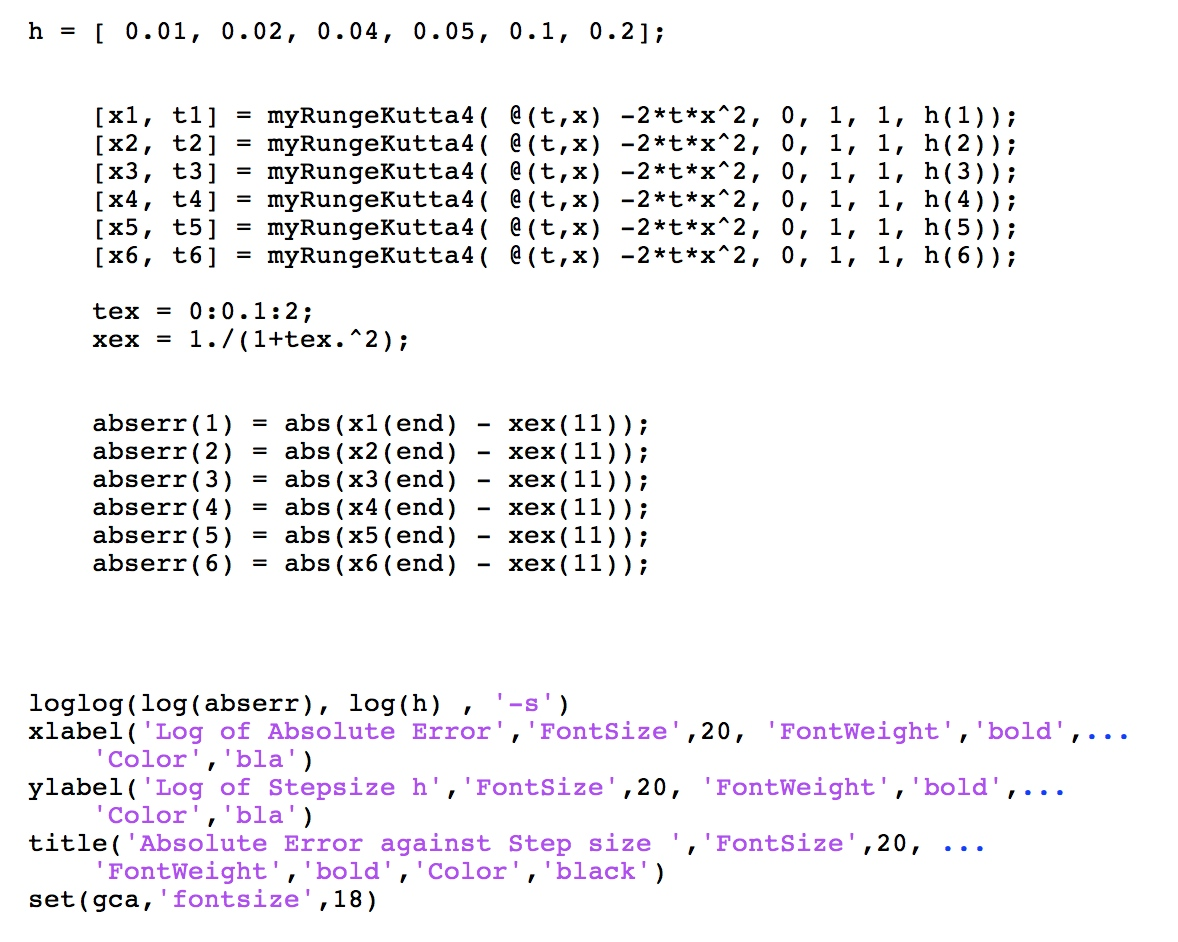
\includegraphics[width=1\textwidth]{rungekuttacodeerrors.jpg}
\end{figure}

The script shown above calls the myRungeKutta4 function for various step sizes $h$, and calculates the absolute error of each against the exact solution. It then plots this on a loglog graph.

%IMAGE - plot of various error sizes(from part 1) vs h calculated from part 1 

\begin{figure}[H]
\centering
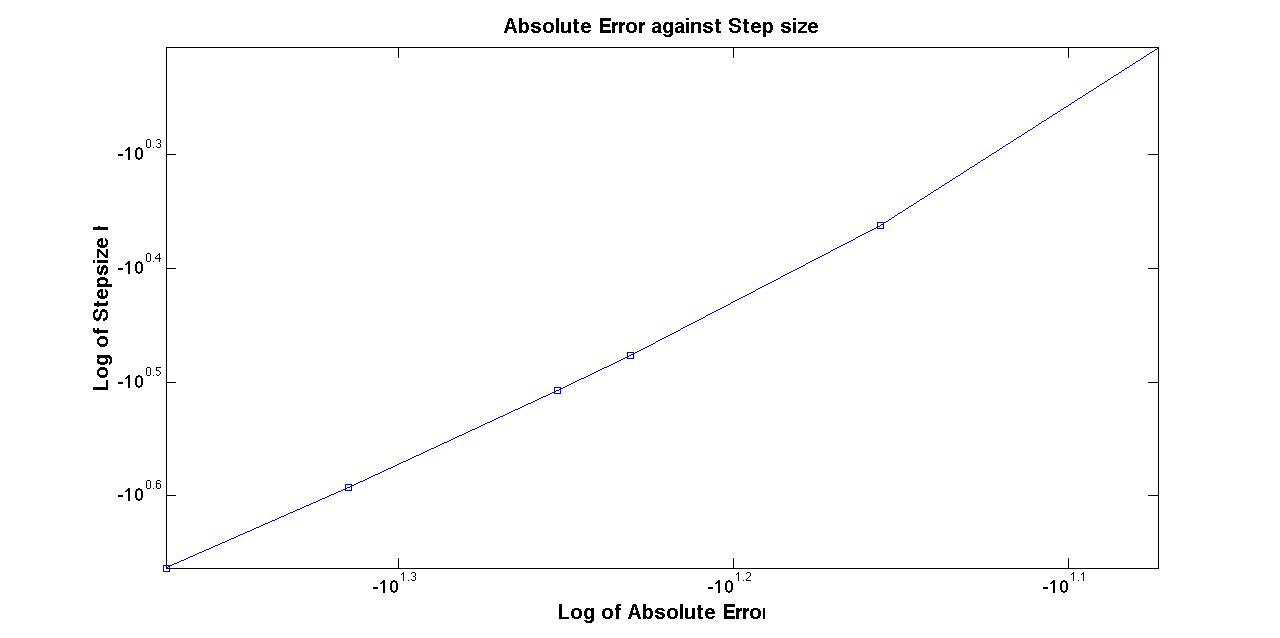
\includegraphics[width=1\textwidth]{rungekuttaerror.jpg}
\caption{\label{fig:rungekuttaerror}A loglog graph showing absolute error vs step size. }
\end{figure}

%Comment on differences between Runge-Kutta and Euler Error

Once again, it can be seen that as the log of the Absolute error increases, as does the log of the stepsize. The errors for Eulers method were $3.6 \times 10^{-4}, 7.1\times 10^{-4}, 1.4\times 10^{-3}, 1.8\times 10^{-3}, 3.6\times 10^{-3}, 7\times 10^{-3}$, and the errors for the Runge-Kutta method are $6.9 \times 10^{-11}, 1.1\times 10^{-9}, 1.7\times 10^{-8}, 4.1\times 10^{-8}, 6\times 10^{-7}, 7.2\times 10^{-6}$ for $h$ of 0.01, 0.02, 0.04, 0.05, 0.1, 0.2 respectively. From this, we can see that the error for the Runge-Kutta method is much lower than the error for Euler's method, and thus fourth order Runge-Kutta is a more accurate method to use.  

\subsection{ODE 45 Right Hand Side Function}

%Explain how ODE45 Works

ODE 45 is a built-in function in Matlab that can solve ODEs. 

%What is the given system of ODEs - math mode system odes
The system of ODEs supplied are:

$$\frac{\mathrm{d}x}{dt} = \alpha(y - x),  \; \; \;   \frac{\mathrm{d}y}{dt} = x(\beta - z),    \; \; \; \frac{\mathrm{d}z}{dt} = xy - \gamma z.$$

%Talk about the parameters/variables

The parameter values that are given are $\alpha = 10, \beta = 350, \gamma = 8/3$, and the initial conditions are $x(0) = 0, y(0) = 50, z(0) = 200$. 

%IMAGE - myODE45 code

\begin{figure}[H]
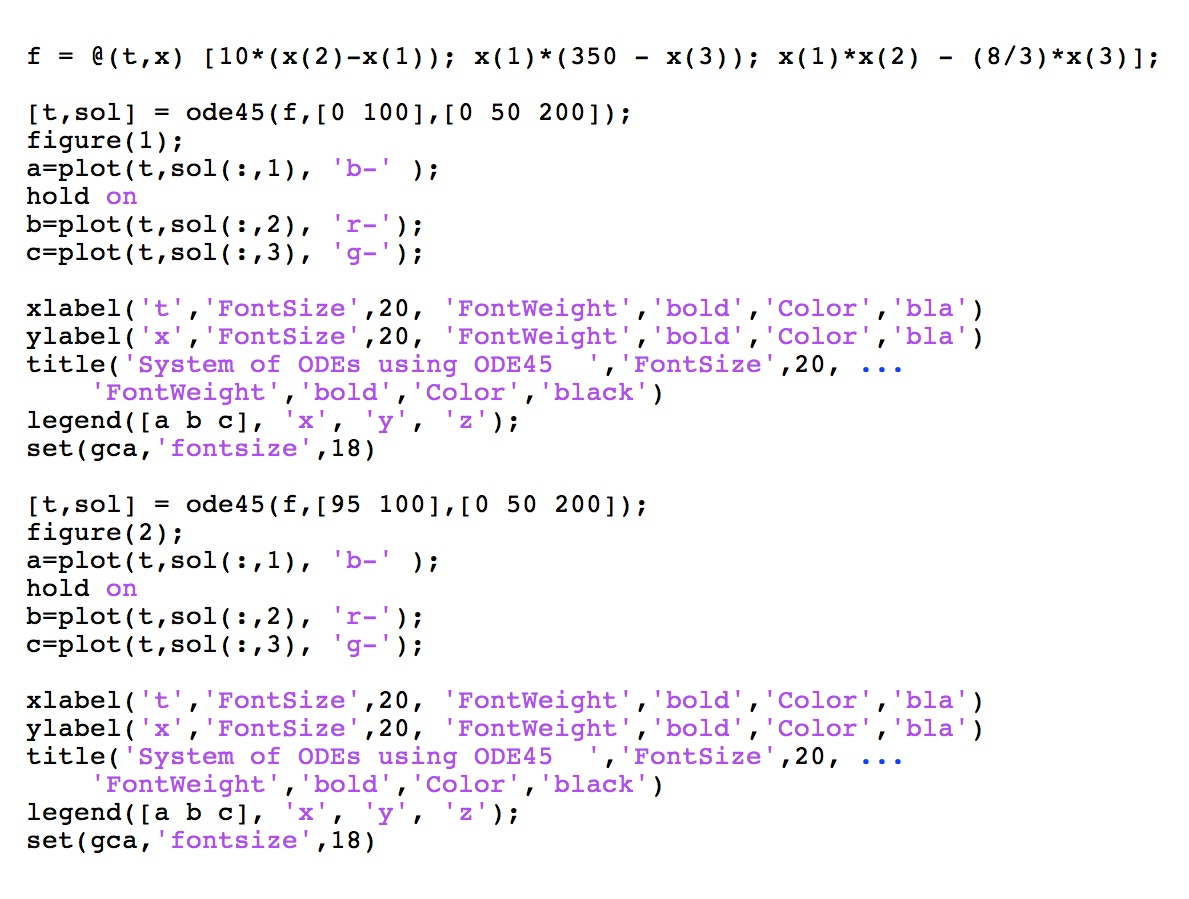
\includegraphics[width=1\textwidth]{ode45code.jpg}
\end{figure}

%Basic explanation of code

In order to use ODE45 to simulate a system of ODEs, what first needs to be done is the three equations need to be put in a vector, called the right hand side function. Then, this function is used in ODE45, along with the initial conditions. This then returns the solution to the system of equations.

%IMAGE - plots of x,y,z v t for t in [0,100]

\begin{figure}[H]
\centering
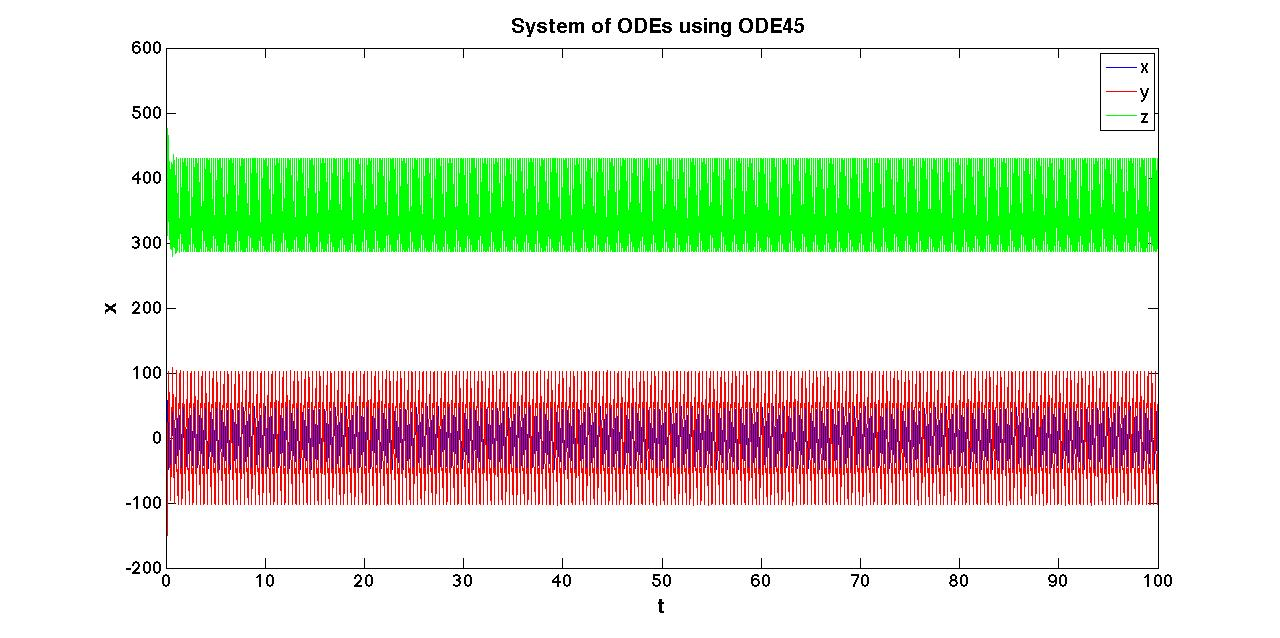
\includegraphics[width=1\textwidth]{ode450to100.jpg}
\caption{\label{fig:ode450to100}A plot of the solution to the system of equations from ODE45 in the timespan $t \in [0, 100].$}
\end{figure}

%IMAGE - plots of x,y,z v t for t in [95,100]

\begin{figure}[H]
\centering
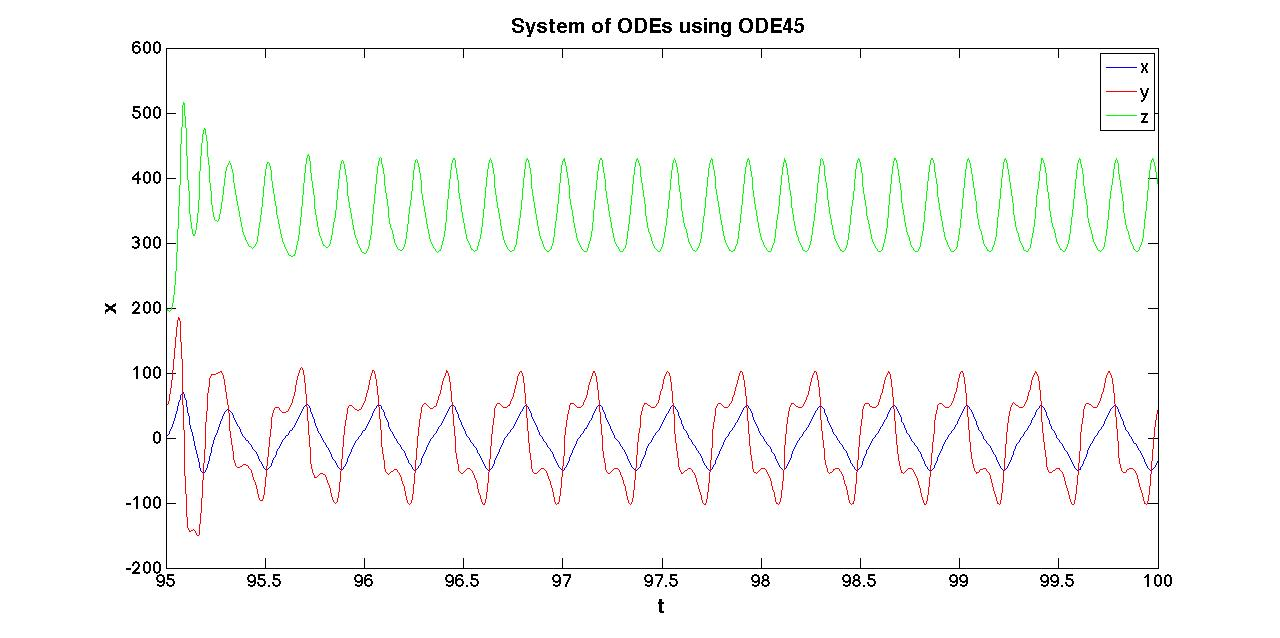
\includegraphics[width=1\textwidth]{ode4595to100.jpg}
\caption{\label{fig:ode4595to100}A plot of the solution to the system of equations from ODE45 in the timespan $t \in [95, 100].$}
\end{figure}

%explain the pattern - what is it, how long does it take to appear, whats the frequency?

As can be seen from both Figure \ref{fig:ode450to100} and Figure \ref{fig:ode4595to100}, there is a visible pattern that can be seen when the solution is plotted. This pattern occurs after around 0.5 seconds, and repeats itself around every 0.4 seconds. 

\section{Numerical Integration}

%What is numerical integration?
Numerical integration is way of solving integrals that doesn't involve manipulating the equation symbolically, rather manipulating the numerical values that the function in the integral gives.

The first choice that needs to be made when writing a function for numerical integration is the method that will be used. I have chosen to use the composite Simpson's rule. 

\subsection{The Composite Simpson's Rule}

%Explain Simpsons rule

%Math mode composite simpsons rule equation

The composite Simpsons rule works by splitting the area upon which the integration must be applied, and using the Simpsons' rule on each area and calculating the total. It uses the following equation:

$$\int_a^b f(x) \, dx\approx\tfrac{h}{3}\bigg[f(x_0)+2\sum_{j=1}^{n/2-1}f(x_{2j})+
4\sum_{j=1}^{n/2}f(x_{2j-1})+f(x_n)\bigg]$$

with $h = \frac{(b-a)}{n}$, and with $n$ being the number of steps that the method should take. 
I chose to use the composite Simpson's rule as it can calculate the integrals of polynomials with order of up to 3 accurately. It is also a fairly simple rule to understand, and it works well for integrals with large limits of integration, as it splits the integrals up. 

%IMAGE - code myNumInt

\subsubsection{The Function}
Below shows the implementation of the composite Simpson's rule in to my numerical integration function. 

\begin{figure}[H]
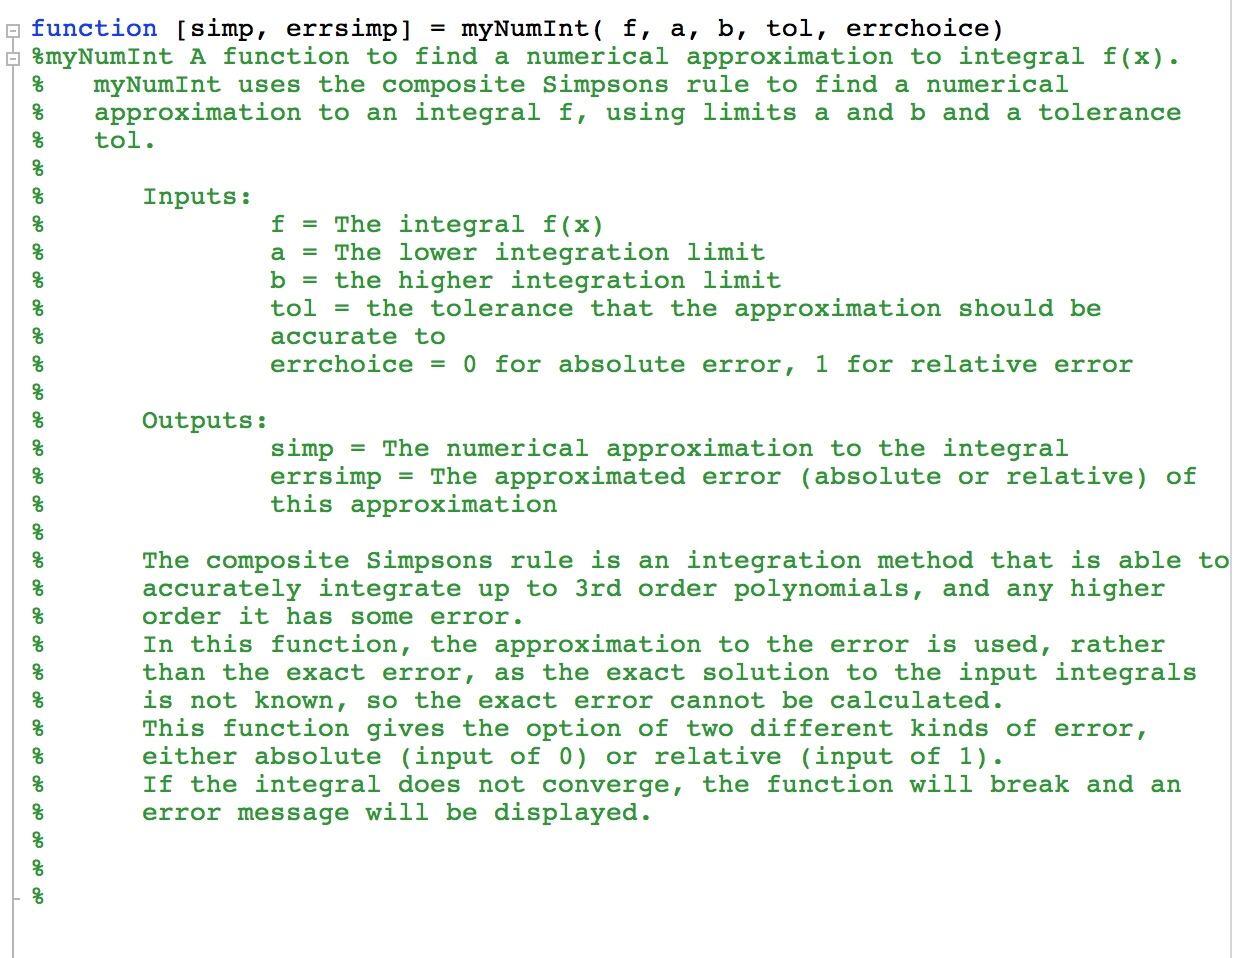
\includegraphics[width=1\textwidth]{mynumint1.jpg}
\end{figure}

The above image shows the help text that I created for using my function. 

\begin{figure}[H]
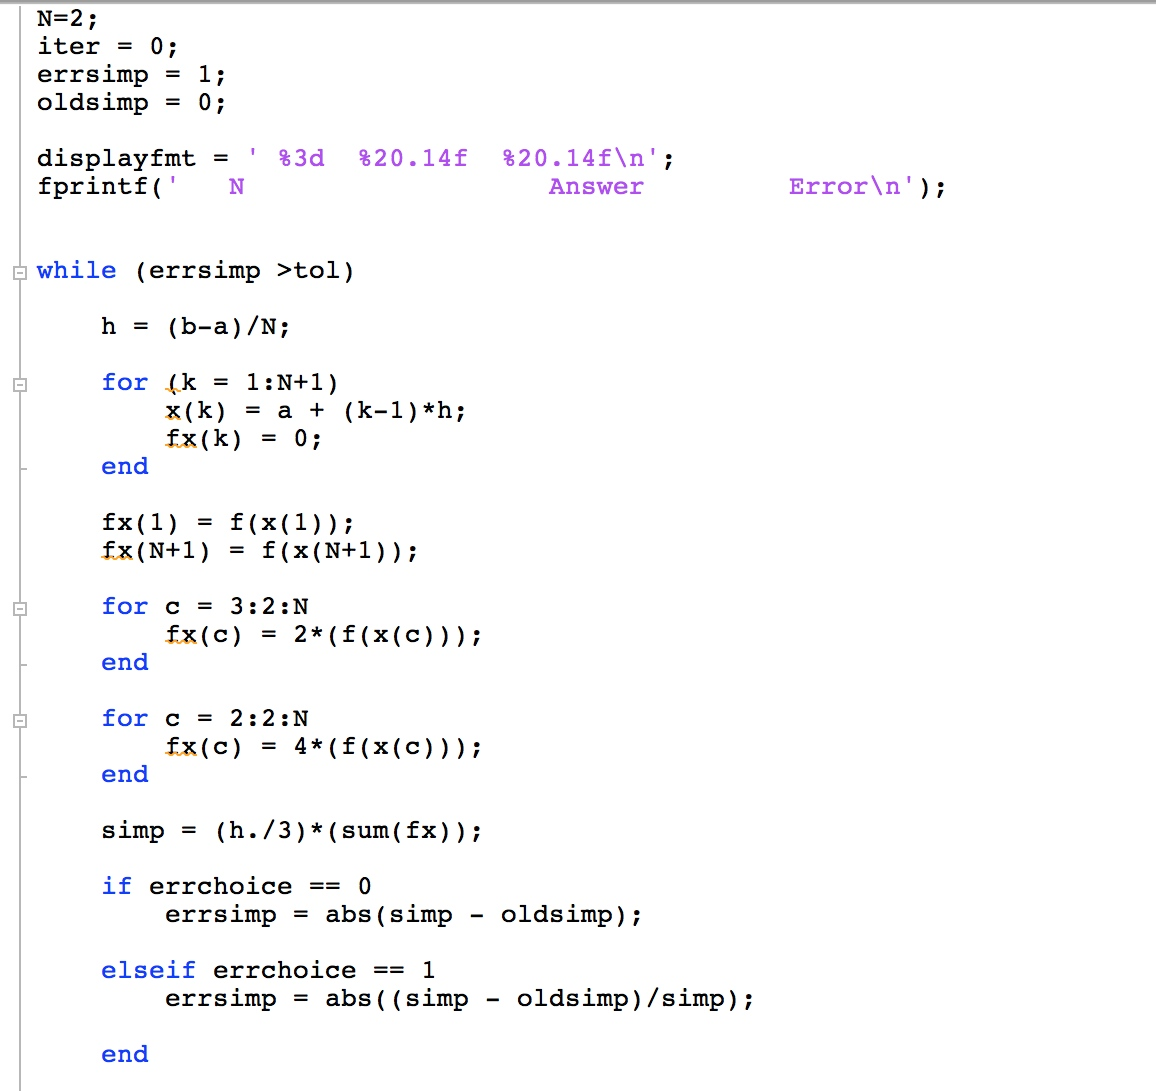
\includegraphics[width=1\textwidth]{mynumint2.jpg}
\end{figure}

The above image shows the while loop used to iterate the composite Simpson's rule, and the way that has been chosen to calculate the values for $f(x)$ when it is needed to be multiplied by two or by four. It also shows the beginning of the grid used to display the information from each iteration. As vectors in Matlab start their index's from 1 rather than 0, it was important to make sure that $f(x_{n+1})$ was used rather than $f(x_{n})$, as this would give the wrong answer, as $f(x_{0})$ is the first term. Hence, $f(x_{2})$ is the first term to be iterated through. 

\begin{figure}[H]
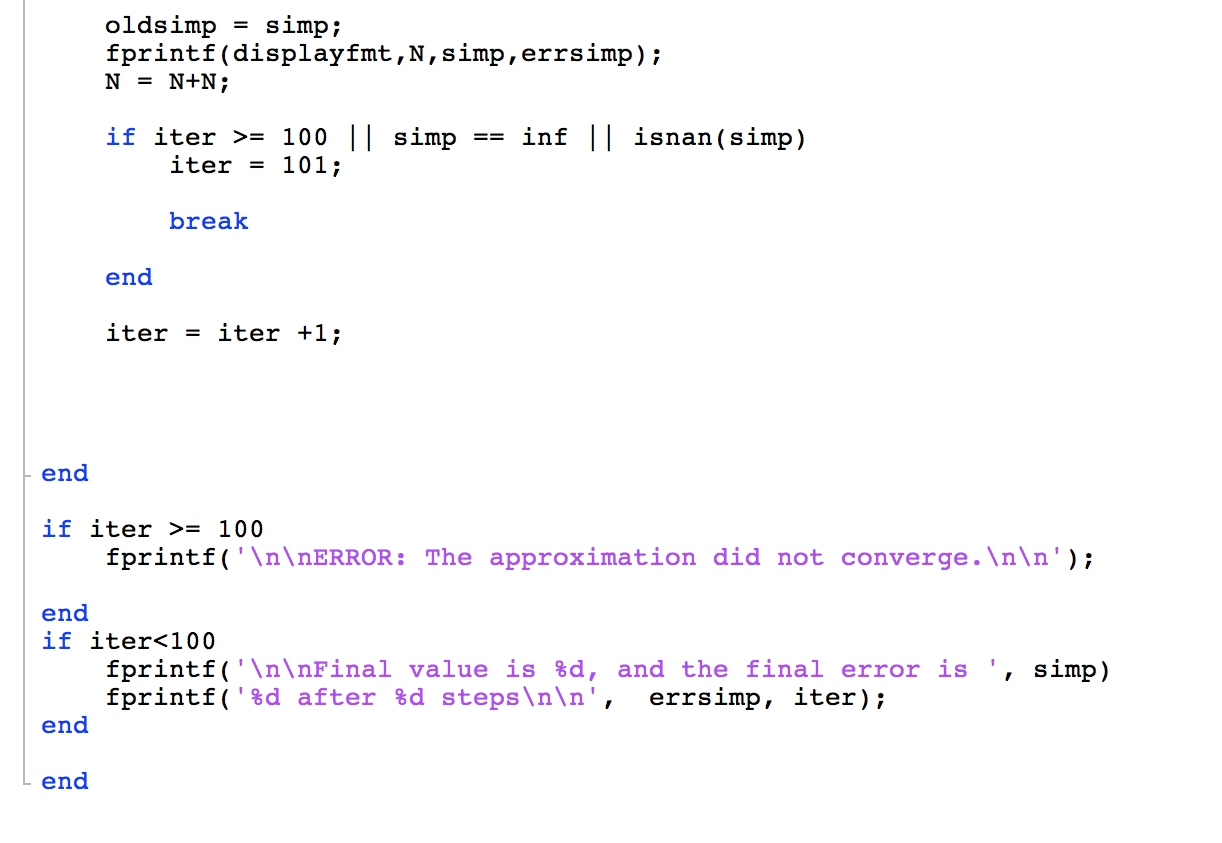
\includegraphics[width=1\textwidth]{mynumint3.jpg}
\end{figure}

This code above shows the second part of the while loop used. It shows the method used to make sure that integrals that do not converge are not left to crash. The break point is chosen as being 100 iterations as if the integral does not converge after this many steps, it is unlikely that it will at all. Infinity is also a cut off point, as is when the solution is not a number. These are so that the function does not crash. 
\newline
Another feature that had to be thought about is the number of steps that the method takes. This was chosen to initially be two, and then to double after every iteration. This is because it wasn't a huge gap between the number of spaces, and if the number of spaces was squared or cubed after each iteration, it would be much larger very quickly, and would take up more time. Doubling $N$ means that it increases at a fairly slow, steady speed, and does not cause the function to crash as much. 




\subsubsection{Testing the Function}

In order to test the function and how well it operated, it is necessary to test it with various different integrals. In order to do this, a script was written that contains various integrals, and the solution to all of these are returned in a single vector.  
%Math mode - integrals to test

%IMAGE - code of integral testing

\begin{figure}[H]
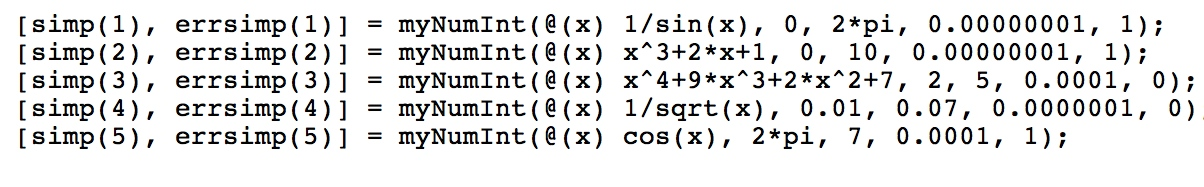
\includegraphics[width=1\textwidth]{numinttest.jpg}
\end{figure}

%What are the outputs from the integrals?

The outputs from these integrals are infinity, $2.61\times 10^3, 2.088\times 10^3, 0.000329\times 10^3 and 0.000657\times 10^3$, and from calculating them by hand the answers are infinity, $2610, 2087.9, 0.32915, 0.65699$, which are incredibly close to the approximations. Therefore, it has been shown that the function is fairly accurate.

%What are the calculated answers, write about the different

\subsection{Solving equation for $\tau$ }

%Explain the problem

The equation given is:

%Math mode - Integral

$$\int_0^\tau \!\frac{1}{\sqrt[3]{1-x^{3}}}\, \mathrm{d}x=1.$$
\newline

%Explain method to solve

In order to solve this using the integration method above, limits must be chosen to work from. To do this, various numbers are input in to the function, and the values that give to closest answer to 1 were chosen. In this case, 0.9 and 0.95 were chosen, as between both of these lies the value of $\tau$ that gives the answer 1. 
\newline \newline

%Explain algorithm

In order to use these values to calculate the correct value of $\tau$, an algorithm must be implemented. This algorithm is shown implemented in the code below.


%IMAGE - code

\begin{figure}[H]
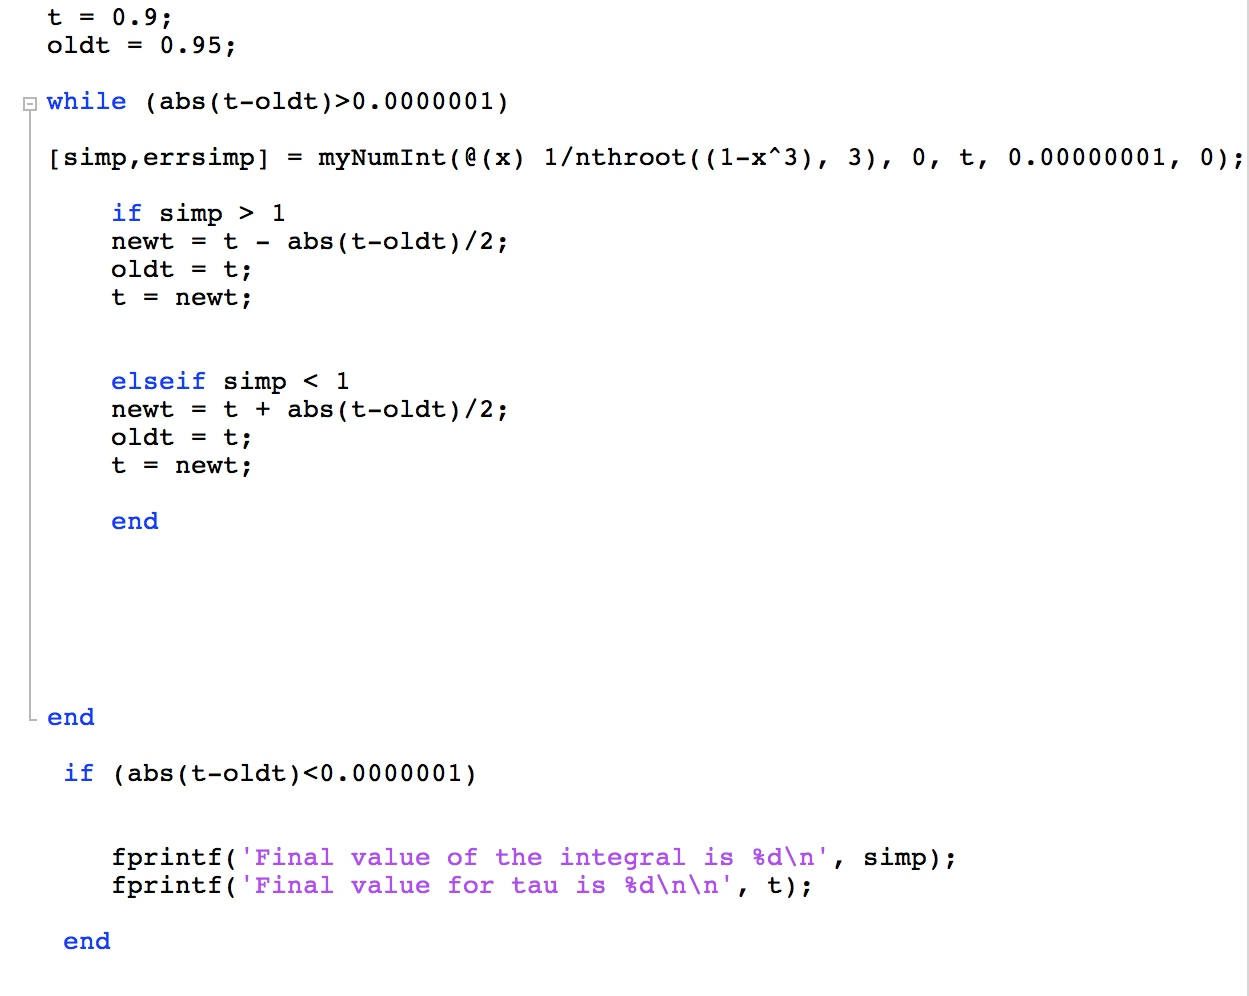
\includegraphics[width=1\textwidth]{codetofindtau.jpg}
\end{figure}

The code works by first setting an initial value of $\tau$, which in this case is 0.9. Then, it checks the approximate absolute error of $\tau$, and if it higher that a certain tolerance (0.0000001 in this case, as $\tau$ is needed to 8 significant figures), it calls the Numerical Integration function that is shown in part 2.1. \newline \newline
After this, the results are used to create a new value for $\tau$, if the approximation is higher than one (the true value of the integral) then the new value of $\tau$ becomes the most recent approximation to $\tau$ minus the difference between the most recent and the older approximation to $\tau$ divided by two, to make the integral approximation decrease. If the approximation is lower than one, the difference between the $\tau$'s divided by two is added to the most recent approximation to $\tau$, in order to make the approximation to the value of the integral increase. This then repeats until the value of $\tau$ is lower than the threshold value.\newline \newline
%Talk about results
The result that was found by running this code had $\tau$ equal to 0.9113923. 


\section{Legendre Polynomials}

\subsection{Recurrence Relation}

%Explain a recurrence relation

A recurrence relation is an equation that uses preceding terms of a sequence to calculate the next term. The recurrence relation supplied is:

%Math mode- recurrence relation

$$nP_n(x)=(2n-1)xP_n-1(x)-(n-1)P_n-2(x),$$ $$ P_0(x)=1, P_1(x)=x.$$
\newline

%IMAGE - code
\begin{figure}[H]
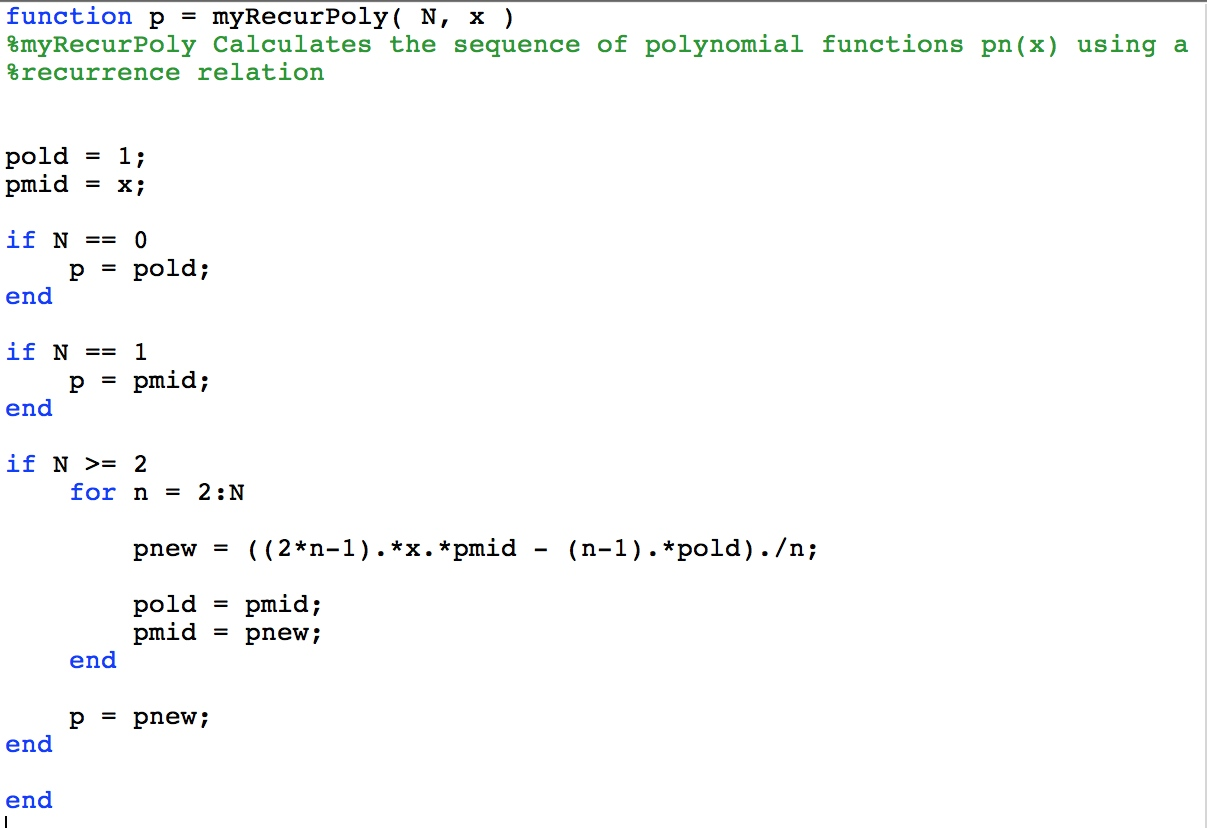
\includegraphics[width=1\textwidth]{recurrencerelationcode.jpg}
\end{figure}

%Explain how the code runs the recurrence relation

\noindent As can be seen from the code above, the only values of the polynomials that need to be stored are the previous two, as they are used to calculate the new polynomial. The code uses inputs of a scalar N, and a vector x. The sequence of polynomial values for the vector x that is input are calculated to degree N. It also has checks to make sure that if the user wants polynomials of either degree 0 or degree 1 there aren't errors, and the correct value is returned.


\subsection{}
\subsection{}
\subsection{}
\subsection{}

\end{document}